\chapter{Growth and Development Accounting}

This chapter transitions from theoretical dynamics to empirical measurement through an exercise known as \textbf{Accounting} (i.e., variance and growth decomposition). The fundamental goal of this chapter is to open the ``black box" of aggregate output and attribute it to observable factors versus unobservable productivity. We ask two distinct quantitative questions:
\begin{enumerate}
    \item \textbf{Development Accounting (Cross-Sectional):} Why are some countries vastly richer than others at a given point in time? How much of this income gap is due to differences in physical and human capital, versus differences in Total Factor Productivity (TFP)?
    \item \textbf{Growth Accounting (Time-Series):} Why does a specific country grow over time? How much of its historical growth rate can be attributed to the accumulation of capital, versus the growth of TFP?
\end{enumerate}

\rmk{
    Typically, empirical evidence suggests that physical capital accumulation accounts for 30-40\% of growth, human capital for about 10\% (though debatable), and the remaining roughly 50\% is attributed to improving productivity.
}

\section{The Production Framework: From General to Specific}

Assume we observe a panel dataset of economies $i \in I$ over time periods $t \in T$:
$$
\{Y_{it}, K_{it}, H_{it}, L_{it}\}_{i\in I, t\in T}
$$
where $Y$ is total output, $K$ is physical capital, $H$ is total human capital (efficiency units of labor, defined later), and $L$ is the raw labor force. 

The aggregate production function is given by:
$$
Y_{it} = A_{it} F(K_{it}, H_{it})
$$
where $F(\cdot)$ is assumed to exhibit \textit{constant returns to scale (CRS)}.

Here, it is crucial to distinguish between the physical properties of the inputs:
\begin{itemize}
    \item \textbf{Rivalrous Inputs ($K_{it}, H_{it}$):} A good is defined as \textit{strictly rivalrous} if its use or consumption by one economic agent fundamentally precludes its simultaneous use by another. Physical capital and human capital are structurally rivalrous because they are strictly bound by physical space and time constraints. For instance, a single machine ($K$) cannot be simultaneously operated by multiple workers without severe congestion. Similarly, human capital ($H$) is embodied within the worker; an hour of a worker's skilled labor deployed in one factory physically cannot be concurrently deployed in another.
    \item \textbf{Non-Rivalrous Productivity ($A_{it}$):} The Total Factor Productivity (TFP) term $A_{it}$ captures non-rivalrous goods—such as knowledge, blueprints, software, and institutional quality. An idea can be shared simultaneously across all workers and machines without being depleted.
\end{itemize}

Because $F(\cdot)$ is CRS, we can divide both sides of the equation by the raw labor force $L_{it}$ to express the economy in per-worker terms. Crucially, because $A_{it}$ is non-rivalrous, this transformation does not dilute it; every worker can fully access the exact same level of technology\footnote{
    Algebraically, because $F(\cdot)$ is CRS, dividing both sides by $L_{it}$ allows us to pass $1/L_{it}$ inside the function $F$, yielding $y_{it} = A_{it} f(k_{it}, h_{it})$. However, this mathematical legality must be strictly backed by the underlying physical properties in economics. 
    
    Imagine if $A_{it}$ were not abstract technology, but rather a pile of ``coal" (a rivalrous good). The original production function would have to be written as $Y_{it} = F(K_{it}, H_{it}, A_{it})$. When converting this economy to per-worker terms, the coal allocated to each worker would inevitably be diluted to $a_{it} = A_{it}/L_{it}$. 
    
    The only reason we are allowed to place $A_{it}$ \textit{outside} the function $F$ as a global multiplier—and completely exempt it from being divided by $L_{it}$ during the per-worker transformation—is because we have predefined technology as strictly non-rivalrous. Regardless of how much the population $L_{it}$ expands, the ``calculus formula" ($A_{it}$) available to each worker remains the complete $A_{it}$, rather than a diluted $A_{it}/L_{it}$.
}.
$$
y_{it} = A_{it} F\left(\frac{K_{it}}{L_{it}}, \frac{H_{it}}{L_{it}}\right) \equiv A_{it} f(k_{it}, h_{it})
$$
where $y_{it}$ is output per worker, $k_{it}$ is physical capital per worker, and $h_{it}$ is human capital per worker.

While the general function $f(\cdot)$ establishes the abstract theoretical mechanics, performing an actual quantitative accounting exercise requires concrete numbers. Specifically, we need to know \textit{by exactly what percentage} output changes when an input changes—this is the output elasticity. To measure and decompose variances in the real-world data, we must parameterize these output elasticities into specific, measurable constants. The universal standard in the macro literature is to adopt the Cobb-Douglas functional form, which conveniently assumes a constant capital share (elasticity) $\alpha \in (0,1)$:
$$
y_{it} = A_{it} k_{it}^{\alpha} h_{it}^{1-\alpha}
$$
Taking the natural logarithm of both sides, we obtain the fundamental log-linearized accounting identity:
$$
\ln y_{it} = \ln A_{it} + \alpha \ln k_{it} + (1-\alpha) \ln h_{it}
$$
This linear additive form is the starting point for all variance and growth decompositions. The fundamental question of macro accounting is: How much of the variation in $\ln y_{it}$ is driven by the observable inputs ($k_{it}, h_{it}$) versus the unobservable TFP residual ($A_{it}$)?

But before we get there, let's take a detour and consider how to pin down $\alpha$ and how to measure human capital $H_{it}$.

\subsection{How to Pin Down $\alpha$?}

To conduct the accounting exercise, we need the value of $\alpha$. A naive approach is to simply run an OLS regression of $\ln y_i$ on $\ln k_i$ and $\ln h_i$ to extract the coefficient. However, this suffers from severe \textit{endogeneity (omitted variable bias)}. The error term $\ln A_i$ is likely to be positively correlated with the regressors (e.g., higher tech countries attract more capital $k_i$), leading OLS to overestimate $\alpha$.

There are typically two ways to cope with this endogeneity problem:
\begin{enumerate}
    \item \textbf{Econometrics:} Find an IV that is orthogonal to $\ln A_i$ and run a 2SLS regression. However, this is often difficult in practice, and the results can be sensitive to the choice of instrument.
    \item \textbf{Economic Theory (The standard approach):} Model the bias away using microeconomics. 
\end{enumerate}

Assuming perfectly competitive markets\footnote{
    In standard microeconomic theory, the assumption of a perfectly competitive market implies that the representative firm is a strict \textit{price taker}. Consequently, the factor prices—the rental rate of capital ($r$) and the wage rate ($w$)—are exogenous and fixed from the firm's perspective. This allows us to equate the marginal product of capital directly to $r$ without modeling the firm's impact on market prices.
}, the representative firm's profit maximization problem is:
\[
\max_{k_i, h_i} A_i k_i^\alpha h_i^{1-\alpha} - r k_i - w h_i
\]
Taking the FOC with respect to $k_i$ gives the marginal product of capital:
\[
\alpha A_i k_i^{\alpha-1} h_i^{1-\alpha} = r \implies \alpha \frac{y_i}{k_i} = r
\]
Rearranging this yields:
\[
\alpha = \frac{r k_i}{y_i}
\]
This elegantly proves that $\alpha$ is exactly equal to the \textit{capital income share} in the national accounts. We can simply look up this share in the data without running any biased regressions.

\subsection{How to Measure Human Capital $h_{it}$?}

Following seminal papers like Hall \& Jones (1999), we construct aggregate human capital by linking macroeconomic aggregates to microeconomic wage data.

Suppose a country has heterogeneous workers divided into schooling groups $j \in \{1, 2, \cdots, J\}$ (e.g., No schooling, Elementary, High school, College). Each group has $s_j$ years of schooling, and makes up a share $l_j$ of the population. Let group 1 be the baseline uneducated workers ($h_1 = 1$). 

Aggregate human capital $H$ is the sum of efficiency units of labor:
\[
H = \sum_{j = 1}^J h_j L_j
\]
This equation converts a heterogeneous workforce into a single, homogeneous macroeconomic measure called ``efficiency units of labor." Specifically, $L_j$ is the absolute number of workers in schooling group $j$, and $h_j$ captures their specific human capital level (or relative productivity weight). By normalizing $h_1 = 1$ for uneducated workers, $H$ essentially measures the total labor input expressed in terms of ``uneducated-worker equivalents."

The firm's problem is to choose capital and the amount of labor from each group to maximize profit:
\[
\max_{K, \{L_j\}} A K^{\alpha} \left(\sum_{j=1}^J h_j L_j\right)^{1-\alpha} - r K - \sum_{j=1}^J w_j L_j
\]
The FOC with respect to labor type $j$ equates the marginal product of labor to its wage:
\[
w_j = (1-\alpha) A K^\alpha H^{-\alpha} \cdot h_j = \left( (1-\alpha)\frac{Y}{H} \right) h_j
\]
By dividing the FOC of group $j$ by the FOC of the uneducated group $1$, we obtain the relative wage ratio:
\[
\frac{w_j}{w_1} = \frac{h_j}{h_1} = h_j
\]
This shows that \textit{relative wages perfectly reflect relative human capital (productivity)}. Thus, the aggregate and per-capita human capital measures $H$ and $h$ can be expressed as\footnote{
    The ``hat" ($\hat{\ }$) explicitly denotes that this is an \textit{empirical estimate} or proxy. The true human capital level $h$ is intrinsically unobservable. However, by leveraging the microeconomic equilibrium condition that wage ratios equal productivity ratios, we can construct the estimator $\hat{h}$ using purely observable market data (relative wages and population shares).
}:
\[
\begin{aligned}
    \hat H & = \sum_{j = 1}^J \left(\frac{w_j}{w_1}\right) L_j\\
\hat{h} & = \sum_{j = 1}^J \left(\frac{w_j}{w_1}\right) l_j
\end{aligned}
\]

\subsection{The Mincer Equation}
How do we find the wage ratio $w_j/w_1$? We rely on the Mincer (1974) wage regression from labor economics:
\[
\ln w_i = m s_i + \beta X_i + \varepsilon_i
\]
Here, $m$ is the \textit{Mincer return}, capturing the percentage wage gain from one additional year of schooling ($s_i$). $X_i$ is a vector of controls. This equation implies:
\[
\ln w_j - \ln w_1 = m(s_j - s_1) \implies \frac{w_j}{w_1} = e^{m(s_j - s_1)}
\]

Substituting the Mincerian wage premium back into our human capital index, we get the final measurement formula:
\[
\hat{h}_{it} = \sum_{j = 1}^J e^{m_{it}(s_{jit} - s_{1it})} l_{jit}
\]
where 
\begin{itemize}
    \item $i$: denotes the specific country (the cross-sectional dimension).
    \item $t$: denotes the specific year (the time-series dimension).
    \item $j$: denotes the specific schooling group within that country and year.
\end{itemize}

To compute this across countries and time, we combine two datasets:
\begin{itemize}
    \item $\{l_{jit}, s_{jit}\}$: Population shares and years of schooling from \textbf{Barro and Lee (2013)}.
    \item $\{m_{it}\}$: Estimates of Mincerian returns to schooling from \textbf{Psacharopoulos \& Patrinos (2018)}.
\end{itemize}

\section{Development Accounting}

Fix a specific year $t$, yielding a cross-sectional dataset $\{y_i, k_i, h_i\}_{i \in I}$. To simplify notation, we aggregate the observable inputs into a single ``factor composite" $X_i$:
\[
X_i \equiv \alpha \ln k_i + (1-\alpha) \ln h_i
\]
Thus, the income variation is perfectly decomposed into observable factors and unobservable TFP:
\[
\ln y_i = X_i + \ln A_i
\]

\begin{itemize}
    \item \textbf{Method 1: The Simple Variance Ratio}\\
    A naive approach measures the contributions as:
\[
s_k^{(1)} = \frac{\Var{\alpha \ln k_i}}{\Var{\ln y_i}}, \quad s_h^{(1)} = \frac{\Var{(1-\alpha) \ln h_i}}{\Var{\ln y_i}}
\]
\textbf{Limitations:} This method has two major statistical flaws. First, variances cannot capture the direction of the relationship. Second, because $\Var{\ln y_i} = \Var{X_i} + \Var{\ln A_i} + 2\Cov{X_i}{\ln A_i}$, the shares will not sum to 100\% unless the covariance between observable factors and TFP is exactly zero (which is strongly rejected in the data).
    \item \textbf{Method 2: Covariance-Based Decomposition}\\
    To address these limitations, the modern literature (e.g., Klenow and Rodríguez-Clare, 1997) universally adopts a covariance-based approach:
\[
s_k = \frac{\Cov{\alpha \ln k_i}{\ln y_i}}{\Var{\ln y_i}}, \quad s_h = \frac{\Cov{(1-\alpha) \ln h_i}{\ln y_i}}{\Var{\ln y_i}}
\]
\textbf{Intuition:} Notice that $s_k$ is exactly the slope coefficient $\beta_k$ from a bivariate OLS regression of $\alpha \ln k_i$ on $\ln y_i$. Furthermore, because covariance is a linear operator, this method equally splits the joint covariance term and elegantly guarantees exact additivity: $s_k + s_h + s_A = 1$ (if we in addition define $s_A = \frac{\Cov{\ln A_i}{\ln y_i}}{\Var{\ln y_i}}$).\footnote{
    By the definition of variance, we know that $\Var{\ln y_i} = \Cov{\ln y_i}{\ln y_i}$. Substituting the income identity $\ln y_i = X_i + \ln A_i$ into the first argument of the covariance yields:
\[
\Var{\ln y_i} = \Cov{X_i + \ln A_i}{\ln y_i} = \Cov{X_i}{\ln y_i} + \Cov{\ln A_i}{\ln y_i}
\]
Dividing both sides by $\Var{\ln y_i}$, we immediately obtain $s_X + s_A = 1$ (where $s_X = s_k + s_h$).
}
\end{itemize}

\section{Growth Accounting}

While development accounting focuses on the cross-country differences in income \textit{levels} at a given point in time, \textit{growth accounting} aims to decompose the changes in income \textit{over time}. 

Suppose we have successfully pinned down the capital share $\alpha$ and observed the panel dataset:
\[
\{y_{it}, k_{it}, h_{it}\}_{i\in I, t\in T}
\]

\subsection{Time-Series Decomposition for a Single Economy}

Pick a specific country $i$ and observe its trajectory over time. We start with the log-linearized production function:
\[
\ln y_{t} = \ln A_t + \alpha \ln k_t + (1-\alpha) \ln h_t
\]
Differentiating across time, we can express this relationship in terms of growth rates:
\[
g_y = g_A + \alpha g_k + (1-\alpha) g_h
\]
where $g_x$ denotes the average growth rate of variable $x$. This additive equation allows us to directly compute the contribution share of each factor to the overall economic growth of that country:
\[
s_k = \frac{\alpha g_k}{g_y}, \quad s_h = \frac{(1-\alpha) g_h}{g_y}, \quad s_A = \frac{g_A}{g_y}
\]
By definition, these shares perfectly sum to 1 (i.e., $s_k + s_h + s_A = 1$).

\rmkb[How to Compute the Average Growth from the Data?]{
    Take the computation of $g_y$ as an example. A naive method is to use the endpoints: $g_y = (\ln y_T - \ln y_0) / T$. However, if the dataset is unbalanced (e.g., missing data for the exact years $0$ or $T$), this method completely fails. Moreover, endpoint calculations are highly sensitive to business cycle fluctuations (e.g., year $T$ happens to be a recession). 

A common practice is to regress the logarithm of the variable on time $t$:
\[
\ln y_t = \beta_0 + g_y \cdot t + \varepsilon_t
\]
The OLS slope coefficient yields a robust estimate of the average growth rate $g_y$. Because OLS utilizes \textit{all} available interior data points to fit the trend line, it elegantly bypasses the issue of missing endpoints and smooths out short-term economic shocks.
\begin{center}
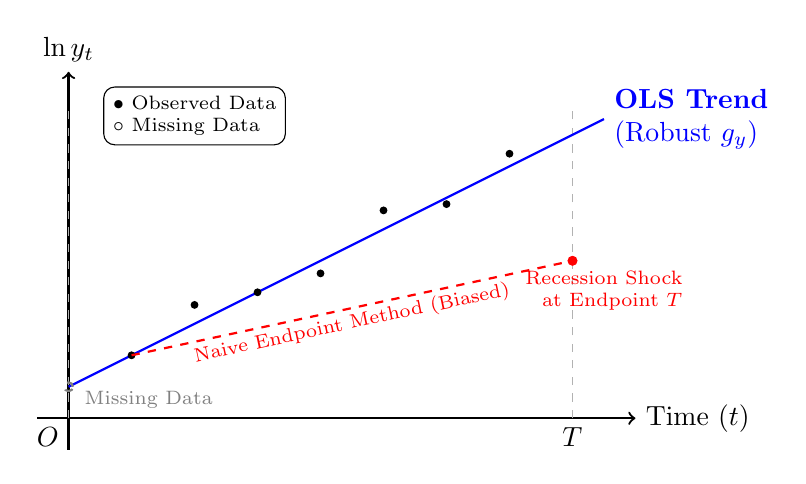
\begin{tikzpicture}[scale=0.8]
    % 坐标轴 (稍微向负方向延伸，打造标准平面直角坐标系的美感)
    \draw[->, thick] (0,-0.5) -- (0,5.5) node[above] {$\ln y_t$};
    \draw[->, thick] (-0.5,0) -- (9.0,0) node[right] {Time ($t$)};
    
    % 原点 O 放置在左下方
    \node[below left] at (0,0) {$O$};
    
    % 标注起点 0 和终点 T
    \draw[dashed, gray!60] (0,0) -- (0,5);
    \draw[dashed, gray!60] (8,0) node[below, text=black] {$T$} -- (8,5);

    % --- 真实的长线增长趋势 (OLS 拟合线) ---
    % 从 (0, 0.5) 到 (8.5, 4.75), 斜率 = 0.5
    \draw[thick, blue] (0, 0.5) -- (8.5, 4.75) node[right, align=left] {\textbf{OLS Trend}\\(Robust $g_y$)};

    % --- 散点数据 (带有经济周期的波动) ---
    % 假设 $t=0$ 数据缺失
    \draw[thick, gray, dashed] (0, 0.5) circle (2pt);
    \node[gray, right, font=\scriptsize] at (0.1, 0.3) {Missing Data};

    % 中间的有效数据点
    \filldraw[black] (1, 1.0) circle (1.5pt);
    \filldraw[black] (2, 1.8) circle (1.5pt); % Boom
    \filldraw[black] (3, 2.0) circle (1.5pt);
    \filldraw[black] (4, 2.3) circle (1.5pt);
    \filldraw[black] (5, 3.3) circle (1.5pt); % Boom
    \filldraw[black] (6, 3.4) circle (1.5pt);
    \filldraw[black] (7, 4.2) circle (1.5pt); % Boom
    
    % $t=T$ 遭遇经济衰退，数据点暴跌，且完美对齐虚线 T
    \filldraw[red] (8, 2.5) circle (2pt); 
    \node[red, below left, font=\scriptsize, align=right] at (9.9, 2.5) {Recession Shock\\at Endpoint $T$};

    % --- 朴素端点法 (Naive Endpoint Method) ---
    % 强行连接现存的第一个点 (t=1) 和最后一个点 (t=T)
    \draw[thick, red, dashed] (1, 1.0) -- (8, 2.5);
    \node[red, rotate=12, font=\scriptsize] at (4.5, 1.5) {Naive Endpoint Method (Biased)};
    
    % 图例说明
    \node[draw, align=left, font=\scriptsize, fill=white, rounded corners] at (2, 4.8) {
        $\bullet$ Observed Data\\
        $\circ$ Missing Data
    };

\end{tikzpicture}
\end{center}
}

\subsection{Cross-Sectional Decomposition of Growth Rates}

The second major question in growth accounting is: \textbf{Why do some countries grow faster than others?} 

To answer this, we shift our focus to the cross-sectional dispersion of growth rates. Suppose we have computed the average growth rates for all countries, yielding the following cross-sectional dataset:
\[
\{g_{y_i}, g_{k_i}, g_{h_i}\}_{i\in I}
\]
Since $g_{y_i} = g_{A_i} + \alpha g_{k_i} + (1-\alpha) g_{h_i}$, we can decompose the \textit{variance} of output growth rates ($\Var{g_{y_i}}$) across countries. The methodology perfectly mirrors development accounting.
\begin{itemize}
    \item \textbf{Method 1: The Simple Variance Ratio} \\
We could naively define the contributions as:
\[
s_k^{(1)} = \frac{\Var{\alpha g_{k_i}}}{\Var{g_{y_i}}}, \quad s_h^{(1)} = \frac{\Var{(1-\alpha) g_{h_i}}}{\Var{g_{y_i}}}
\]
As discussed in Development Accounting, this method is statistically flawed. Because input growth rates and TFP growth are often correlated (e.g., fast technological adoption induces rapid capital accumulation), the covariance terms are non-zero. Consequently, the shares under Method 1 will not sum up to 100\%.
    \item \textbf{Method 2: Covariance-Based Decomposition} \\
To ensure exact additivity, the standard literature employs the covariance-based approach:
\[
s_k = \frac{\Cov{\alpha g_{k_i}}{g_{y_i}}}{\Var{g_{y_i}}}, \quad s_h = \frac{\Cov{(1-\alpha) g_{h_i}}{g_{y_i}}}{\Var{g_{y_i}}}, \quad s_A = \frac{\Cov{g_{A_i}}{g_{y_i}}}{\Var{g_{y_i}}}
\]
\textbf{Intuition:} Once again, $s_k$ can be perfectly visualized as the slope coefficient from an OLS regression of the capital contribution ($\alpha g_{k_i}$) on the overall growth rate ($g_{y_i}$). This method dynamically allocates the covariance between factor accumulation and technological progress, guaranteeing that $s_k + s_h + s_A = 1$.
\end{itemize}

